% $Author: oscar $
% $Date: 2009-09-15 16:53:48 +0200 (Tue, 15 Sep 2009) $
% $Revision: 29111 $
%=================================================================
\ifx\wholebook\relax\else
% --------------------------------------------
% Lulu:
	\documentclass[a4paper,10pt,twoside]{book}
	\usepackage[
		papersize={6.13in,9.21in},
		hmargin={.815in,.815in},
		vmargin={.98in,.98in},
		ignoreheadfoot
	]{geometry}
	% $Author: oscar $
% $Date: 2009-09-13 20:58:29 +0200 (Sun, 13 Sep 2009) $
% $Revision: 29070 $
%=============================================================
% NB: documentclass must be set in main document.
% Allows book to be generated in multiple formats.
%=============================================================
%:Packages
\usepackage[T1]{fontenc}  %%%%%really important to get the code directly in the text!
\usepackage{palatino}
\usepackage{ifthen}
\usepackage{graphicx}
\graphicspath{{figures/}}
\usepackage{xspace}
\usepackage{makeidx}
\usepackage{isodateo} % enable \isodate
\usepackage{amssymb,textcomp}
%=============================================================
%:More packages
%\usepackage[english]{babel}
%\usepackage{lmodern}
%\usepackage[scaled=0.85]{helvet}
%\usepackage{microtype}
%\usepackage{theorem}
%\usepackage{float}
%\usepackage{longtable}
%\usepackage[nottoc]{tocbibind}
%\usepackage{multicol}
%\usepackage{booktabs}	% book-style tables
%\usepackage{topcapt}	% enables \topcaption
%\usepackage{multirow}
%\usepackage{tabularx}
%\usepackage{alltt}
\usepackage[usenames,dvipsnames]{color}
%\usepackage[hang]{subfigure}\makeatletter\def\p@subfigure{\thefigure\,}\makeatother
%\usepackage{rotating}
%\usepackage{enumitem}	% apb: allows more control over tags in enumerations
%\usepackage{verbatim}     % for comment environment
%\usepackage{varioref}	% for page references that work
%\usepackage{needspace}
%\usepackage[newparttoc]{titlesec}
%\usepackage{titletoc}
%\usepackage{wrapfig}
\usepackage[
	colorlinks=true,
	linkcolor=black,
	urlcolor=black,
	citecolor=black
]{hyperref}   % should come last
%=============================================================
%:URL style
\makeatletter
\def\url@leostyle{%
  \@ifundefined{selectfont}{\def\UrlFont{\sf}}{\def\UrlFont{\sffamily}}}
\makeatother
\urlstyle{leo}
%=============================================================
%:Booleans
\newboolean{lulu}
\setboolean{lulu}{false}
\newcommand{\ifluluelse}[2]{\ifthenelse{\boolean{lulu}}{#1}{#2}}
%=============================================================
%:Editorial comment macros
\newcommand{\nnbb}[2]{
  \fbox{\bfseries\sffamily\scriptsize#1}
  {\sf\small$\blacktriangleright$\textit{#2}$\blacktriangleleft$}
}
\newcommand{\on}[1]{\nnbb{Oscar}{#1}}
\newcommand{\here}{\nnbb{CONTINUE}{HERE}}
%=============================================================
%:Abbreviation macros
\newcommand{\ie}{\emph{i.e.},\xspace}
\newcommand{\eg}{\emph{e.g.},\xspace}
\newcommand{\etc}{\emph{etc.}\xspace}
\newcommand{\etal}{\emph{et al.}\xspace}
\newcommand{\straightquote}{"}
\newcommand{\sba}{\url{SquareBracketAssociates.org}\xspace}
%=============================================================
%:Patterns
% \newcommand{\pattern}[2]{\newpage\section{{\sf #1}}\label{pat:#2}}
% \newcommand{\pattern}[2]{\newpage\index{#1 (Pattern)}\section{#1}\label{pat:#2}}
\newcommand{\pattern}[2]{\cleardoublepage\index{#1 (패턴)}\section{#1}\label{pat:#2}}
\newcommand{\thumbnail}[2]{\index{#1 (패턴)}\subsection{#1}\label{pat:#2}}
\newcommand{\thumblang}[2]{\index{#1 (패턴 랭귀지)}\subsection{#1}\label{pat:#2}}
\newcommand{\variant}[1]{{\emph{#1}}\xspace}
% \newcommand{\problem}[1]{\subsection*{Problem}\emph{#1}}
\newcommand{\intent}[1]{\paragraph{의도}\emph{#1}}
\newcommand{\problem}[1]{\paragraph{문제}\emph{#1}}
\newcommand{\solution}[1]{\paragraph{해결}\emph{#1}}
\newcommand{\discussion}[0]{\paragraph{토론}}
\newcommand{\cmd}[1]{{\tt #1}\xspace}
%=============================================================
%:Environments
\newenvironment{bulletlist}{\begin{itemize}\setlength{\itemsep}{0ex}}
{\end{itemize}}
%=============================================================
%:Cross reference macros
\newcommand{\chalabel}[1]{\label{cha:#1}}
\newcommand{\seclabel}[1]{\label{sec:#1}}
\newcommand{\figlabel}[1]{\label{fig:#1}}
\newcommand{\tablabel}[1]{\label{tab:#1}}
\newcommand{\rulelabel}[1]{\label{rule:#1}}
\newcommand{\eglabel}[1]{\label{eg:#1}}
\newcommand{\scrlabel}[1]{\label{scr:#1}}
\newcommand{\mthlabel}[1]{\label{mth:#1}}
\newcommand{\clslabel}[1]{\label{cls:#1}}
\newcommand{\faqlabel}[1]{\label{faq:#1}}
%\newcommand{\charef}[1]{Chapter~\ref{cha:#1}\xspace}
%\newcommand{\secref}[1]{Section~\ref{sec:#1}\xspace}
\newcommand{\figref}[1]{Figure~\ref{fig:#1}\xspace}
% \newcommand{\patpgref}[2]{\hyperref[pat:#2]{\sf #1} [p.~\pageref{pat:#2}]\xspace}
\newcommand{\patpgref}[2]{\index{#1 (Pattern)}\hyperref[pat:#2]{#1} [p.~\pageref{pat:#2}]\xspace}
\newcommand{\patlangpgref}[2]{\index{#1 (Pattern language)}\hyperref[pat:#2]{#1} [p.~\pageref{pat:#2}]\xspace}
% \newcommand{\patref}[2]{\hyperref[pat:#2]{\sf #1}\xspace}
\newcommand{\patref}[2]{\index{#1 (Pattern)}\hyperref[pat:#2]{#1}\xspace}
\newcommand{\patlangref}[2]{\index{#1 (Pattern language)}\hyperref[pat:#2]{#1}\xspace}
% \newcommand{\charef}[2]{\hyperref[cha:#2]{\underline{\sf #1}}\xspace}
% \newcommand{\charef}[2]{\hyperref[cha:#2]{\sf #1}\xspace}
\newcommand{\charef}[2]{\index{#1 (Pattern cluster)}\hyperref[cha:#2]{#1}\xspace}
% \newcommand{\chapgref}[2]{\hyperref[cha:#2]{\sf #1} [p.~\pageref{cha:#2}]\xspace}
\newcommand{\chapgref}[2]{\index{#1 (Pattern cluster)}\hyperref[cha:#2]{#1} [p.~\pageref{cha:#2}]\xspace}
%\newcommand{\Figref}[1]{Figure~\ref{fig:#1}\xspace}
%\newcommand{\appref}[1]{Appendix~\ref{app:#1}\xspace}
%\newcommand{\tabref}[1]{Table~\ref{tab:#1}\xspace}
%\newcommand{\ruleref}[1]{\ref{rule:#1}\xspace}
%\newcommand{\egref}[1]{example~\ref{eg:#1}\xspace}
%\newcommand{\Egref}[1]{Example~\ref{eg:#1}\xspace}
%\newcommand{\scrref}[1]{script~\ref{scr:#1}\xspace}
%\newcommand{\Scrref}[1]{Script~\ref{scr:#1}\xspace}
%\newcommand{\tscrref}[1]{the script~\ref{scr:#1}\xspace}
%\newcommand{\Tscrref}[1]{The script~\ref{scr:#1}\xspace}
%\newcommand{\mthref}[1]{method~\ref{mth:#1}\xspace}
%\newcommand{\mthsref}[1]{methods~\ref{mth:#1}\xspace}
%\newcommand{\Mthref}[1]{Method~\ref{mth:#1}\xspace}
%\newcommand{\tmthref}[1]{the method~\ref{mth:#1}\xspace}
%\newcommand{\Tmthref}[1]{The method~\ref{mth:#1}\xspace}
%\newcommand{\clsref}[1]{class~\ref{cls:#1}\xspace}
%\newcommand{\tclsref}[1]{the class~\ref{cls:#1}\xspace}
%\newcommand{\Tclsref}[1]{The class~\ref{cls:#1}\xspace}
%=============================================================
%:Page Layout
\setlength{\headsep}{1cm}
%=============================================================
%:Menu item macro
%\definecolor{lightgray}{gray}{0.89}
%\newcommand{\menu}[1]{{%
%	\setlength{\fboxsep}{0pt}%
%	\colorbox{lightgray}{{{\upshape\sffamily\strut \,#1\,}}}}}
%\newcommand{\go}{\,$\triangleright$\,}
%\newcommand{\short}[1]{\mbox{{\sc cmd}\hspace{0.08em}--\hspace{0.09em}#1}\xspace}
%\newcommand{\button}[1]{{%
%	\setlength{\fboxsep}{0pt}%
%	\fbox{{\upshape\sffamily\strut \,#1\,}}}}
%\newcommand{\toolsflap}{\textit{Tools} flap\xspace}
%=============================================================
%:Section depth
%\setcounter{secnumdepth}{2}
%
%\DeclareGraphicsExtensions{.pdf, .jpg, .png}
%=============================================================
%:PDF setup
\hypersetup{
   pdftitle={Object-Oriented Reengineering Patterns},
   pdfauthor={Serge Demeyer, St\'ephane Ducasse, Oscar Nierstrasz},
   pdfkeywords={Reengineering, Object-Oriented Programming, Patterns},
   pdfsubject={Computer Science}
}
%=============================================================
%:Page layout and appearance
%\renewcommand{\chaptermark}[1]{\markboth{#1}{}}
%\renewcommand{\sectionmark}[1]{\markright{\thesection\ #1}}
%\renewpagestyle{plain}[\small\itshape]{%
%	\setheadrule{0pt}%
%	\sethead[][][]{}{}{}%
%	\setfoot[][][]{}{}{}}
%\renewpagestyle{headings}[\small\itshape]{%
%	\setheadrule{0pt}%
%	\setmarks{chapter}{section}%
%	\sethead[\thepage][][\chaptertitle]{\sectiontitle}{}{\thepage}%
%	\setfoot[][][]{}{}{}}
%=============================================================
%:Title section setup and TOC numbering depth
%\setcounter{secnumdepth}{1}
%\setcounter{tocdepth}{1}
%\titleformat{\part}[display]{\centering}{\huge\partname\ \thepart}{1em}{\Huge\textbf}[]
%\titleformat{\chapter}[display]{}{\huge\chaptertitlename\ \thechapter}{1em}{\Huge\raggedright\textbf}[]
%\titlecontents{part}[3pc]{%
%		\pagebreak[2]\addvspace{1em plus.4em minus.2em}%
%		\leavevmode\large\bfseries}
%	{\contentslabel{3pc}}{\hspace*{-3pc}}
%	{}[\nopagebreak]
%\titlecontents{chapter}[3pc]{%
%		\pagebreak[0]\addvspace{1em plus.2em minus.2em}%
%		\leavevmode\bfseries}
%	{\contentslabel{3pc}}{}
%	{\hfill\contentspage}[\nopagebreak]
%\dottedcontents{section}[3pc]{}{3pc}{1pc}
%\dottedcontents{subsection}[3pc]{}{0pc}{1pc}
%\let\origdoublepage\cleardoublepage
%\newcommand{\clearemptydoublepage}{%
%  \clearpage
%  {\pagestyle{empty}\origdoublepage}}
%\let\cleardoublepage\clearemptydoublepage % see http://www.tex.ac.uk/cgi-bin/texfaq2html?label=patch
%=============================================================
%:Listings package configuration
\newcommand{\caret}{\makebox{\raisebox{0.4ex}{\footnotesize{$\wedge$}}}}
% \newcommand{\escape}{{\sf \textbackslash}}
\definecolor{source}{gray}{0.95}
\usepackage{listings}
\lstdefinelanguage{Smalltalk}{
  morestring=[d]',
% Adapt this to other languages!
%  morecomment=[s]{"}{"},
  alsoletter={\#:},
  %escapechar={!},
  literate=
    {BANG}{!}1
%    {UNDERSCORE}{\_}1
    {\\st}{Smalltalk}9 % convenience -- in case \st occurs in code
    % {'}{{\textquotesingle}}1 % replaced by upquote=true in \lstset
%    {_}{{$\leftarrow$}}1
    {>>>}{{\sep}}1
    {^}{{$\uparrow$}}1
    {~}{{$\sim$}}1
    {-}{{\sf -\hspace{-0.13em}-}}1  % the goal is to make - the same width as +
    {+}{\raisebox{0.08ex}{+}}1		% and to raise + off the baseline to match -
    {-->}{{\quad$\longrightarrow$\quad}}3
	, % Don't forget the comma at the end!
  tabsize=4
}[keywords,comments,strings]

\lstset{language=Smalltalk,
	basicstyle=\sffamily,
	keywordstyle=\color{black}\bfseries,
	% stringstyle=\ttfamily, % Ugly! do we really want this? -- on
	mathescape=true,
	showstringspaces=false,
	keepspaces=true,
	breaklines=true,
	breakautoindent=true,
	backgroundcolor=\color{source},
	lineskip={-1pt}, % Ugly hack
	upquote=true, % straight quote; requires textcomp package
	columns=fullflexible} % no fixed width fonts
% \newcommand{\ct}{\lstinline[mathescape=false,basicstyle={\sffamily\upshape}]}
\newcommand{\ct}{\lstinline[mathescape=false,backgroundcolor=\color{white},basicstyle={\sffamily\upshape}]}
\newcommand{\lct}[1]{{\textsf{\textup{#1}}}}
%\newcommand{\scat}[1]{\emph{\textsf{#1}}\xspace}
%\newcommand{\prot}[1]{\emph{\textsf{#1}}\xspace}
% NB: No argument!
\lstnewenvironment{code}[0]{%
	\lstset{%
		% frame=lines,
		frame=single,
		framerule=0pt,
		mathescape=false
	}
}{}
%\def\ignoredollar#1{}
%=============================================================
%:Reserving space
%\newcommand{\needlines}[1]{\Needspace{#1\baselineskip}}
%=============================================================
%:Indexing macros
% Macros ending with "ind" generate text as well as an index entry
% Macros ending with "index" *only* generate an index entry
\newcommand{\ind}[1]{\index{#1}#1\xspace} % plain text
\newcommand{\subind}[2]{\index{#1!#2}#2\xspace} % show #2, subindex under #1
\newcommand{\emphind}[1]{\index{#1}\emph{#1}\xspace} % emph #1
\newcommand{\emphsubind}[2]{\index{#1!#2}\emph{#2}\xspace} % show emph #2, subindex under #1
\newcommand{\patind}[1]{\index{#1@#1 (pattern)}\ct{#1}\xspace} % pattern
\newcommand{\seeindex}[2]{\index{#1|see{#2}}} % #1, see #2
%\newcommand{\boldidx}[1]{{\bf #1}} % breaks hyperlink
%\newcommand{\indmain}[1]{\index{#1}#1\xspace} 
%\newcommand{\emphsubindmain}[2]{\index{#1!#2}\emph{#2}\xspace} % subindex, main entry
%\newcommand{\subindmain}[2]{\index{#1!#2}#2\xspace} % subindex, main entry
%\newcommand{\clsindmain}[1]{\index{#1!\#@(class)}\ct{#1}\xspace} % class main
%\newcommand{\indexmain}[1]{\index{#1}} 
%=============================================================
\parskip 1ex
%=============================================================

	\pagestyle{headings}
	\setboolean{lulu}{true}
	\usepackage[hangul]{kotex}
% --------------------------------------------
% A4:
%	\documentclass[a4paper,11pt,twoside]{book}
%	% $Author: oscar $
% $Date: 2009-09-13 20:58:29 +0200 (Sun, 13 Sep 2009) $
% $Revision: 29070 $
%=============================================================
% NB: documentclass must be set in main document.
% Allows book to be generated in multiple formats.
%=============================================================
%:Packages
\usepackage[T1]{fontenc}  %%%%%really important to get the code directly in the text!
\usepackage{palatino}
\usepackage{ifthen}
\usepackage{graphicx}
\graphicspath{{figures/}}
\usepackage{xspace}
\usepackage{makeidx}
\usepackage{isodateo} % enable \isodate
\usepackage{amssymb,textcomp}
%=============================================================
%:More packages
%\usepackage[english]{babel}
%\usepackage{lmodern}
%\usepackage[scaled=0.85]{helvet}
%\usepackage{microtype}
%\usepackage{theorem}
%\usepackage{float}
%\usepackage{longtable}
%\usepackage[nottoc]{tocbibind}
%\usepackage{multicol}
%\usepackage{booktabs}	% book-style tables
%\usepackage{topcapt}	% enables \topcaption
%\usepackage{multirow}
%\usepackage{tabularx}
%\usepackage{alltt}
\usepackage[usenames,dvipsnames]{color}
%\usepackage[hang]{subfigure}\makeatletter\def\p@subfigure{\thefigure\,}\makeatother
%\usepackage{rotating}
%\usepackage{enumitem}	% apb: allows more control over tags in enumerations
%\usepackage{verbatim}     % for comment environment
%\usepackage{varioref}	% for page references that work
%\usepackage{needspace}
%\usepackage[newparttoc]{titlesec}
%\usepackage{titletoc}
%\usepackage{wrapfig}
\usepackage[
	colorlinks=true,
	linkcolor=black,
	urlcolor=black,
	citecolor=black
]{hyperref}   % should come last
%=============================================================
%:URL style
\makeatletter
\def\url@leostyle{%
  \@ifundefined{selectfont}{\def\UrlFont{\sf}}{\def\UrlFont{\sffamily}}}
\makeatother
\urlstyle{leo}
%=============================================================
%:Booleans
\newboolean{lulu}
\setboolean{lulu}{false}
\newcommand{\ifluluelse}[2]{\ifthenelse{\boolean{lulu}}{#1}{#2}}
%=============================================================
%:Editorial comment macros
\newcommand{\nnbb}[2]{
  \fbox{\bfseries\sffamily\scriptsize#1}
  {\sf\small$\blacktriangleright$\textit{#2}$\blacktriangleleft$}
}
\newcommand{\on}[1]{\nnbb{Oscar}{#1}}
\newcommand{\here}{\nnbb{CONTINUE}{HERE}}
%=============================================================
%:Abbreviation macros
\newcommand{\ie}{\emph{i.e.},\xspace}
\newcommand{\eg}{\emph{e.g.},\xspace}
\newcommand{\etc}{\emph{etc.}\xspace}
\newcommand{\etal}{\emph{et al.}\xspace}
\newcommand{\straightquote}{"}
\newcommand{\sba}{\url{SquareBracketAssociates.org}\xspace}
%=============================================================
%:Patterns
% \newcommand{\pattern}[2]{\newpage\section{{\sf #1}}\label{pat:#2}}
% \newcommand{\pattern}[2]{\newpage\index{#1 (Pattern)}\section{#1}\label{pat:#2}}
\newcommand{\pattern}[2]{\cleardoublepage\index{#1 (패턴)}\section{#1}\label{pat:#2}}
\newcommand{\thumbnail}[2]{\index{#1 (패턴)}\subsection{#1}\label{pat:#2}}
\newcommand{\thumblang}[2]{\index{#1 (패턴 랭귀지)}\subsection{#1}\label{pat:#2}}
\newcommand{\variant}[1]{{\emph{#1}}\xspace}
% \newcommand{\problem}[1]{\subsection*{Problem}\emph{#1}}
\newcommand{\intent}[1]{\paragraph{의도}\emph{#1}}
\newcommand{\problem}[1]{\paragraph{문제}\emph{#1}}
\newcommand{\solution}[1]{\paragraph{해결}\emph{#1}}
\newcommand{\discussion}[0]{\paragraph{토론}}
\newcommand{\cmd}[1]{{\tt #1}\xspace}
%=============================================================
%:Environments
\newenvironment{bulletlist}{\begin{itemize}\setlength{\itemsep}{0ex}}
{\end{itemize}}
%=============================================================
%:Cross reference macros
\newcommand{\chalabel}[1]{\label{cha:#1}}
\newcommand{\seclabel}[1]{\label{sec:#1}}
\newcommand{\figlabel}[1]{\label{fig:#1}}
\newcommand{\tablabel}[1]{\label{tab:#1}}
\newcommand{\rulelabel}[1]{\label{rule:#1}}
\newcommand{\eglabel}[1]{\label{eg:#1}}
\newcommand{\scrlabel}[1]{\label{scr:#1}}
\newcommand{\mthlabel}[1]{\label{mth:#1}}
\newcommand{\clslabel}[1]{\label{cls:#1}}
\newcommand{\faqlabel}[1]{\label{faq:#1}}
%\newcommand{\charef}[1]{Chapter~\ref{cha:#1}\xspace}
%\newcommand{\secref}[1]{Section~\ref{sec:#1}\xspace}
\newcommand{\figref}[1]{Figure~\ref{fig:#1}\xspace}
% \newcommand{\patpgref}[2]{\hyperref[pat:#2]{\sf #1} [p.~\pageref{pat:#2}]\xspace}
\newcommand{\patpgref}[2]{\index{#1 (Pattern)}\hyperref[pat:#2]{#1} [p.~\pageref{pat:#2}]\xspace}
\newcommand{\patlangpgref}[2]{\index{#1 (Pattern language)}\hyperref[pat:#2]{#1} [p.~\pageref{pat:#2}]\xspace}
% \newcommand{\patref}[2]{\hyperref[pat:#2]{\sf #1}\xspace}
\newcommand{\patref}[2]{\index{#1 (Pattern)}\hyperref[pat:#2]{#1}\xspace}
\newcommand{\patlangref}[2]{\index{#1 (Pattern language)}\hyperref[pat:#2]{#1}\xspace}
% \newcommand{\charef}[2]{\hyperref[cha:#2]{\underline{\sf #1}}\xspace}
% \newcommand{\charef}[2]{\hyperref[cha:#2]{\sf #1}\xspace}
\newcommand{\charef}[2]{\index{#1 (Pattern cluster)}\hyperref[cha:#2]{#1}\xspace}
% \newcommand{\chapgref}[2]{\hyperref[cha:#2]{\sf #1} [p.~\pageref{cha:#2}]\xspace}
\newcommand{\chapgref}[2]{\index{#1 (Pattern cluster)}\hyperref[cha:#2]{#1} [p.~\pageref{cha:#2}]\xspace}
%\newcommand{\Figref}[1]{Figure~\ref{fig:#1}\xspace}
%\newcommand{\appref}[1]{Appendix~\ref{app:#1}\xspace}
%\newcommand{\tabref}[1]{Table~\ref{tab:#1}\xspace}
%\newcommand{\ruleref}[1]{\ref{rule:#1}\xspace}
%\newcommand{\egref}[1]{example~\ref{eg:#1}\xspace}
%\newcommand{\Egref}[1]{Example~\ref{eg:#1}\xspace}
%\newcommand{\scrref}[1]{script~\ref{scr:#1}\xspace}
%\newcommand{\Scrref}[1]{Script~\ref{scr:#1}\xspace}
%\newcommand{\tscrref}[1]{the script~\ref{scr:#1}\xspace}
%\newcommand{\Tscrref}[1]{The script~\ref{scr:#1}\xspace}
%\newcommand{\mthref}[1]{method~\ref{mth:#1}\xspace}
%\newcommand{\mthsref}[1]{methods~\ref{mth:#1}\xspace}
%\newcommand{\Mthref}[1]{Method~\ref{mth:#1}\xspace}
%\newcommand{\tmthref}[1]{the method~\ref{mth:#1}\xspace}
%\newcommand{\Tmthref}[1]{The method~\ref{mth:#1}\xspace}
%\newcommand{\clsref}[1]{class~\ref{cls:#1}\xspace}
%\newcommand{\tclsref}[1]{the class~\ref{cls:#1}\xspace}
%\newcommand{\Tclsref}[1]{The class~\ref{cls:#1}\xspace}
%=============================================================
%:Page Layout
\setlength{\headsep}{1cm}
%=============================================================
%:Menu item macro
%\definecolor{lightgray}{gray}{0.89}
%\newcommand{\menu}[1]{{%
%	\setlength{\fboxsep}{0pt}%
%	\colorbox{lightgray}{{{\upshape\sffamily\strut \,#1\,}}}}}
%\newcommand{\go}{\,$\triangleright$\,}
%\newcommand{\short}[1]{\mbox{{\sc cmd}\hspace{0.08em}--\hspace{0.09em}#1}\xspace}
%\newcommand{\button}[1]{{%
%	\setlength{\fboxsep}{0pt}%
%	\fbox{{\upshape\sffamily\strut \,#1\,}}}}
%\newcommand{\toolsflap}{\textit{Tools} flap\xspace}
%=============================================================
%:Section depth
%\setcounter{secnumdepth}{2}
%
%\DeclareGraphicsExtensions{.pdf, .jpg, .png}
%=============================================================
%:PDF setup
\hypersetup{
   pdftitle={Object-Oriented Reengineering Patterns},
   pdfauthor={Serge Demeyer, St\'ephane Ducasse, Oscar Nierstrasz},
   pdfkeywords={Reengineering, Object-Oriented Programming, Patterns},
   pdfsubject={Computer Science}
}
%=============================================================
%:Page layout and appearance
%\renewcommand{\chaptermark}[1]{\markboth{#1}{}}
%\renewcommand{\sectionmark}[1]{\markright{\thesection\ #1}}
%\renewpagestyle{plain}[\small\itshape]{%
%	\setheadrule{0pt}%
%	\sethead[][][]{}{}{}%
%	\setfoot[][][]{}{}{}}
%\renewpagestyle{headings}[\small\itshape]{%
%	\setheadrule{0pt}%
%	\setmarks{chapter}{section}%
%	\sethead[\thepage][][\chaptertitle]{\sectiontitle}{}{\thepage}%
%	\setfoot[][][]{}{}{}}
%=============================================================
%:Title section setup and TOC numbering depth
%\setcounter{secnumdepth}{1}
%\setcounter{tocdepth}{1}
%\titleformat{\part}[display]{\centering}{\huge\partname\ \thepart}{1em}{\Huge\textbf}[]
%\titleformat{\chapter}[display]{}{\huge\chaptertitlename\ \thechapter}{1em}{\Huge\raggedright\textbf}[]
%\titlecontents{part}[3pc]{%
%		\pagebreak[2]\addvspace{1em plus.4em minus.2em}%
%		\leavevmode\large\bfseries}
%	{\contentslabel{3pc}}{\hspace*{-3pc}}
%	{}[\nopagebreak]
%\titlecontents{chapter}[3pc]{%
%		\pagebreak[0]\addvspace{1em plus.2em minus.2em}%
%		\leavevmode\bfseries}
%	{\contentslabel{3pc}}{}
%	{\hfill\contentspage}[\nopagebreak]
%\dottedcontents{section}[3pc]{}{3pc}{1pc}
%\dottedcontents{subsection}[3pc]{}{0pc}{1pc}
%\let\origdoublepage\cleardoublepage
%\newcommand{\clearemptydoublepage}{%
%  \clearpage
%  {\pagestyle{empty}\origdoublepage}}
%\let\cleardoublepage\clearemptydoublepage % see http://www.tex.ac.uk/cgi-bin/texfaq2html?label=patch
%=============================================================
%:Listings package configuration
\newcommand{\caret}{\makebox{\raisebox{0.4ex}{\footnotesize{$\wedge$}}}}
% \newcommand{\escape}{{\sf \textbackslash}}
\definecolor{source}{gray}{0.95}
\usepackage{listings}
\lstdefinelanguage{Smalltalk}{
  morestring=[d]',
% Adapt this to other languages!
%  morecomment=[s]{"}{"},
  alsoletter={\#:},
  %escapechar={!},
  literate=
    {BANG}{!}1
%    {UNDERSCORE}{\_}1
    {\\st}{Smalltalk}9 % convenience -- in case \st occurs in code
    % {'}{{\textquotesingle}}1 % replaced by upquote=true in \lstset
%    {_}{{$\leftarrow$}}1
    {>>>}{{\sep}}1
    {^}{{$\uparrow$}}1
    {~}{{$\sim$}}1
    {-}{{\sf -\hspace{-0.13em}-}}1  % the goal is to make - the same width as +
    {+}{\raisebox{0.08ex}{+}}1		% and to raise + off the baseline to match -
    {-->}{{\quad$\longrightarrow$\quad}}3
	, % Don't forget the comma at the end!
  tabsize=4
}[keywords,comments,strings]

\lstset{language=Smalltalk,
	basicstyle=\sffamily,
	keywordstyle=\color{black}\bfseries,
	% stringstyle=\ttfamily, % Ugly! do we really want this? -- on
	mathescape=true,
	showstringspaces=false,
	keepspaces=true,
	breaklines=true,
	breakautoindent=true,
	backgroundcolor=\color{source},
	lineskip={-1pt}, % Ugly hack
	upquote=true, % straight quote; requires textcomp package
	columns=fullflexible} % no fixed width fonts
% \newcommand{\ct}{\lstinline[mathescape=false,basicstyle={\sffamily\upshape}]}
\newcommand{\ct}{\lstinline[mathescape=false,backgroundcolor=\color{white},basicstyle={\sffamily\upshape}]}
\newcommand{\lct}[1]{{\textsf{\textup{#1}}}}
%\newcommand{\scat}[1]{\emph{\textsf{#1}}\xspace}
%\newcommand{\prot}[1]{\emph{\textsf{#1}}\xspace}
% NB: No argument!
\lstnewenvironment{code}[0]{%
	\lstset{%
		% frame=lines,
		frame=single,
		framerule=0pt,
		mathescape=false
	}
}{}
%\def\ignoredollar#1{}
%=============================================================
%:Reserving space
%\newcommand{\needlines}[1]{\Needspace{#1\baselineskip}}
%=============================================================
%:Indexing macros
% Macros ending with "ind" generate text as well as an index entry
% Macros ending with "index" *only* generate an index entry
\newcommand{\ind}[1]{\index{#1}#1\xspace} % plain text
\newcommand{\subind}[2]{\index{#1!#2}#2\xspace} % show #2, subindex under #1
\newcommand{\emphind}[1]{\index{#1}\emph{#1}\xspace} % emph #1
\newcommand{\emphsubind}[2]{\index{#1!#2}\emph{#2}\xspace} % show emph #2, subindex under #1
\newcommand{\patind}[1]{\index{#1@#1 (pattern)}\ct{#1}\xspace} % pattern
\newcommand{\seeindex}[2]{\index{#1|see{#2}}} % #1, see #2
%\newcommand{\boldidx}[1]{{\bf #1}} % breaks hyperlink
%\newcommand{\indmain}[1]{\index{#1}#1\xspace} 
%\newcommand{\emphsubindmain}[2]{\index{#1!#2}\emph{#2}\xspace} % subindex, main entry
%\newcommand{\subindmain}[2]{\index{#1!#2}#2\xspace} % subindex, main entry
%\newcommand{\clsindmain}[1]{\index{#1!\#@(class)}\ct{#1}\xspace} % class main
%\newcommand{\indexmain}[1]{\index{#1}} 
%=============================================================
\parskip 1ex
%=============================================================

%	\usepackage{a4wide}
% --------------------------------------------
	\begin{document}
	% \renewcommand{\nnbb}[2]{} % Disable editorial comments
	\sloppy
\fi
%=================================================================
\chapter{리엔지니어링 패턴}
\chalabel{ReengineeringPatterns}

%=================================================================
\section{왜 리엔지니어링인가?}

유산(레거시, legacy)이란 \emph{물려받은 것} 중에 \emph{가치가 있는 것}이다. 마찬가지로, \ind{레거시 소프트웨어}는 여러분이 물려받은 가치 있는 소프트웨어이다. 상속받았다는 것은 다소 구식이라는 것을 의미할 수 있다. 오래된 프로그래밍 언어나 구식 개발 방법을 사용하여 개발되었을 수 있다. 개발자가 여러 번 바뀌었고 많은 수정과 변형의 흔적이 남아 있을 가능성이 높다. 

어쩌면 레거시 소프트웨어가 그렇게 오래되지 않았을 수도 있다. 빠른 개발 도구와 인력의 빠른 이직으로 인해 소프트웨어 시스템은 상상 이상으로 빠르게 레거시가 될 수 있다. 하지만 소프트웨어의 \emph{가치가 높다}는 사실은 이를 그냥 버릴 수 없다는 것을 의미한다. 

레거시 소프트웨어는 비즈니스에 매우 중요하며, 이것이 바로 모든 문제의 근원이다. 비즈니스에서 성공하려면 변화하는 비즈니스 환경에 적응할 수 있도록 끊임없이 준비해야 한다. 따라서 비즈니스를 운영하는 데 사용하는 소프트웨어도 적응력이 있어야 한다. 다행히도 많은 소프트웨어는 업그레이드할 수 있고, 더 이상 쓸모가 없어지면 간단히 폐기하고 교체할 수도 있다. 하지만 레거시 시스템은 많은 비용이 들지 않는 한 교체하거나 업그레이드할 수 없다. 리엔지니어링의 목표는 레거시 시스템의 복잡성을 충분히 줄여 적절한 비용으로 계속 사용하고 적응할 수 있도록 하는 것이다. 

소프트웨어 시스템을 리엔지니어링해야 하는 구체적인 이유는 매우 다양할 수 있다. 예를 들어 다음과 같다.
\begin{bulletlist}
  \item 개별 파트를 더 쉽게 개별적으로 판매하거나 다른 방식으로 결합할 수 있도록 모놀리식 시스템(monolithic system)을 \emph{언번들링(unbundle)}\footnote{그룹으로 되어 있던 제품 및 서비스 패키지를 분리하는 프로세스 -옮긴이}하려고 할 수 있다.

  \item \emph{성능(performance)}을 개선하고 싶을 수 있다. (경험상 올바른 순서는 ``먼저 동작하게 하고, 제대로 동작하게 하고, 빠르게 동작하게 하는 것(first do it, then do it right, then do it fast)''이므로 성능에 대해 생각하기 전에 코드를 정리하는 리엔지니어링을 하는 것이 좋다.)

  \item \emph{시스템을 새 플랫폼으로 포팅(port the system to a new platform)}하고 싶을 수도 있다. 그 전에 플랫폼에 종속된 코드를 명확하게 분리하기 위해 아키텍처를 변경해야 할 수도 있다.

  \item 새롭게 구현하는 첫 번째 단계로 \emph{디자인 추출(extract the design)}을 수행할 수 있다.

  \item 유지보수 비용을 절감하기 위한 단계로 새로운 표준이나 라이브러리와 같은 \emph{신기술을 활용(exploit new technology)}하고 싶을 수도 있다.
  
  \item 시스템에 대한 지식을 문서화하여 유지보수를 더 쉽게 함으로써 \emph{인적 종속성을 줄이려고(reduce human dependencies)} 할 수도 있다.
\end{bulletlist}

시스템을 리엔지니어링하는 데에는 여러 가지 이유가 있을 수 있다. 앞으로 살펴보겠지만 레거시 소프트웨어의 실제 기술적 문제는 매우 유사한 경우가 많다. 이러한 사실 덕분에 리엔지니어링 작업의 일부분이라도 매우 일반적인 기술을 사용할 수 있다.

%-----------------------------------------------------------------
\subsection*{리엔지니어링 필요성 인식}

레거시 문제가 있는지 어떻게 알 수 있을까? 

``고장 나지 않았으면 고치지 말자(If it ain't broke, don't fix it.)''는 것이 일반적인 통념이다. 이러한 태도는 종종 중요한 기능을 수행하고 있고 잘 작동하는 것처럼 보이는 소프트웨어에 손을 대지 않으려는 핑계로 받아들여진다. 이 접근 방식의 문제점은 무언가가 ``고장''날 수 있는 방법이 다양하다는 점을 인식하지 못한다는 것이다. 기능적인 관점는, 무언가는 설계된 바데로 기능을 더 이상 수행하지 못하는 경우에만 고장난 것이다. 그러나 유지 관리 관점에서 보면 소프트웨어는 \emph{더 이상 유지 관리할 수 없는 경우} 고장난 것이다.

그렇다면 소프트웨어가 곧 고장날 것이라는 것을 어떻게 알 수 있을까? 다행히도 문제가 발생하고 있다는 것을 알려주는 경고 신호가 많이 있다. 아래 나열된 증상은 일반적으로 단독으로 발생하는 것이 아니라 한 번에 여러 개씩 나타난다. 

\begin{description}
  \item[문서가 없거나 더 이상 사용되지 않음(Obsolete or no documentation).] \index{문서!폐기}
사용되지 않는 문서는 많은 변화를 겪은 레거시 시스템의 분명한 신호이다. 문서가 없다는 것은 원래 개발자가 프로젝트를 떠나자마자 문제가 발생할 수 있다는 경고 신호이다.

  \item[테스트 누락(Missing tests).] \index{테스트! 누락}
최신 문서보다 더 중요한 것은 모든 시스템 구성 요소에 대한 철저한 단위 테스트와 모든 중요한 사용 사례 및 시나리오를 포괄하는 시스템 테스트의 존재 여부이다. 이러한 테스트가 없다는 것은 시스템이 높은 위험이나 비용 없이 발전할 수 없다는 신호이다.

  \item[기존 개발자 또는 사용자의 이동(Original developers or users have left).]
테스트 커버리지가 좋은 깨끗하고 잘 문서화된 시스템이 아니라면, 그보다 훨씬 덜 깨끗하고 문서화가 잘 안 된 시스템으로 급속히 악화될 것이다.

  \item[사라진 시스템의 내부 지식(Inside knowledge about system has disappeared).]
이것은 나쁜 신호이다. 문서가 기존 코드 베이스와 동기화되지 않는다. 아무도 실제로 어떻게 작동하는지 모른다.

  \item[제한적 전체 시스템 이해(Limited understanding of the entire system).]
아무도 상세 내용을 이해하지 못할 뿐만 아니라 전체 시스템에 대해 제대로 파악하고 있는 사람도 거의 없다. 

  \item[상용화 시간이 오래 걸림(Too long to turn things over to production).]
프로세스의 어딘가에 문제가 있다. 변경 사항을 승인하는 데 너무 오래 걸리는 것일 수 있다. 자동 회귀 테스트가 누락되었을 수도 있다. 또는 변경 사항을 배포하기가 어려울 수도 있다. 이러한 어려움을 이해하고 대처하지 않으면 상황은 더욱 악화될 것이다.

  \item[간단한 변경에 너무 많은 시간이 소요(Too much time to make simple changes).]
이것은 리먼과 벨레이디의 \ind{복잡성 증가의 법칙(Law of Increasing Complexity)}이 시작되었다는 분명한 신호이다. 이제 시스템이 너무 복잡해져서 간단한 변경조차 구현하기 어렵다는 뜻이다. 시스템을 간단하게 변경하는 데 너무 오랜 시간이 걸리면 복잡한 변경을 하는 것은 당연히 불가능할 것이다. 간단한 변경이 완료되기를 기다리는 백로그가 있으면 어려운 문제를 해결할 수 없다.

  \item[줄어들지 않는 버그(Need for constant bug fixes).]
버그는 절대 사라지지 않는 것 같다. 버그를 수정할 때마다 그 옆에 새로운 버그가 나타난다. 이는 애플리케이션의 일부가 너무 복잡해져서 더 이상 작은 변경의 영향을 정확하게 평가할 수 없다는 것을 의미한다. 또한 애플리케이션의 아키텍처가 더 이상 요구 사항과 일치하지 않으므로 작은 변경도 예기치 않은 결과를 초래할 수 있다.

  \item[유지 관리 종속성(Maintenance Dependencies).]
한 곳에서 버그를 수정하면 다른 곳에서 또 다른 버그가 \emph{다른 곳에} 나타난다. 이는 종종 시스템의 논리적으로 분리된 구성 요소가 더 이상 독립적이지 않을 정도로 아키텍처가 악화되었다는 신호이다. 

  \item[오래 걸리는 빌드 시간(Big build times).]
재컴파일 시간이 길면 변경 작업이 느려진다. 빌드 시간이 길다는 것은 시스템 구성이 너무 복잡해서 컴파일러 툴이 효율적으로 작동하지 않는다는 의미일 수도 있다. 

  \item[어려운 제품 분리(Difficulties separating products).]
제품에 대한 고객이 많고 각 고객에 맞게 릴리스를 조정하는 데 어려움이 있다면 아키텍처가 더 이상 작업에 적합하지 않은 것이다.

  \item[중복된 코드(Duplicated code)] \index{중복된 코드}
중복 코드는 시스템이 발전함에 따라 자연스럽게 발생하며, 거의 동일한 코드를 구현하거나 소프트웨어 시스템의 여러 버전을 병합하는 지름길로 사용된다. 공통 부분을 적절한 추상화로 리팩토링하여 중복 코드를 제거하지 않으면 동일한 코드를 여러 곳에서 수정해야 하므로 유지 관리가 점점 어려워 질 수 있다.

  \item[코드 스멜(Code Smells).] \index{코드 스멜}\index{벡, 켄트}
중복된 코드는 ``나쁜 냄새''가 나므로 변경해야 하는 코드의 예이다. 긴 메서드, 큰 클래스, 긴 매개변수 목록, 스위치 문, 데이터 클래스 등은 켄트 벡과 다른 사람들이 문서화한 몇 가지 예이다 \cite{Fowl99a}. 코드 스멜은 종종 시스템이 재설계되지 않은 채 반복적으로 확장되고 조정되었다는 신호이다.

\end{description}

%-----------------------------------------------------------------
\subsection*{객체의 특별한 점}

이 책에서 설명하는 많은 기술이 모든 소프트웨어 시스템에 적용될 수 있지만, 저자들은 \emph{객체 지향 레거시 시스템}에 초점을 맞추기로 했다. 이러한 선택에는 여러 가지 이유가 있지만, 무엇보다도 많은 객체 지향 기술 얼리 어답터들이 객체로 전환함으로써 기대했던 이점을 실현하기가 매우 어려웠다는 사실을 발견하고 있는 중요한 시점이라고 생각했기 때문이다.

이제 \ind{Java}에도 레거시 시스템이 상당히 많이 존재한다. 소프트웨어가 레거시 시스템으로 변하는 것은 \emph{시간(age)}가 아니라 재설계되지 않고 개발 및 적용되어 온 \emph{정도(rate)}이다.

이러한 경험에서 도출할 수 있는 잘못된 결론은 ``객체가 좋지 않아 다른 것이 필요하다''는 것이다. 이미 우리는 패턴, 컴포넌트, UML, XMI 등 많은 새로운 트렌드를 향해 달려가는 것을 목격하고 있다. 이러한 발전 중 모두 좋은 것이지만 어떤 의미에서는 모두 요점을 놓치고 있다.

이 책에서 얻을 수 있는 결론 중 하나는 객체는 꽤 좋지만 \emph{``객체를 잘 관리해야 한다''}는 것이다. 이 점을 이해하려면 유연성(flexibility), 유지보수성(maintainability), 재사용성(reuse)이 그토록 좋은 객체 지향 시스템에서 왜 레거시 문제가 발생하는지 생각해 보자.

우선, 기존의 객체 지향 코드 베이스로 작업해 본 사람이라면 누구나 눈치챘을 것아다: \emph{객체를 찾기가 어렵다}라는 부분이다. 실제로 객체 지향 애플리케이션의 아키텍처는 일반적으로 숨겨져 있다. 눈에 보이는 것은 여러 개의 클래스와 상속 계층 구조뿐이다. 하지만 런타임에 어떤 객체가 존재하고 어떻게 협업하여 원하는 동작을 제공하는지는 알 수 없다. 객체 지향 시스템을 이해하는 것은 리버스 엔지니어링의 과정이며, 이 책에서 설명하는 기법은 이 문제를 해결하는 데 도움이 된다. 또한 코드를 리엔지니어링하면 아키텍처를 이해하기 쉬운 더 투명한 시스템에 도달할 수 있다.

\index{소프트웨어 재사용}
둘째, 기존 객체 지향 애플리케이션을 확장해 본 사람이라면 누구나 깨달았을 것이다: \emph{재사용은 공짜로 얻을 수 없다}. 실제로 코드를 재사용할 수 있도록 설계하는 데 상당한 노력을 기울이지 않는 한 코드를 재사용하는 것은 매우 어렵다. 또한 재사용에 대한 투자는 올바른 조직 인프라를 구축하기 위한 경영진의 의지가 필수적이며, 명확하고 측정 가능한 목표를 염두에 두고 수행해야 한다 \cite{Gold95a}.

우리는 아직 재사용을 적절히 고려하는 방식으로 객체 지향 소프트웨어 프로젝트를 관리하는 데 능숙하지 않다. 일반적으로 재사용은 너무 늦게 이루어진다. 우리는 객체 지향 모델링 기법을 사용하여 매우 풍부하고 복잡한 객체 모델을 개발하고, 소프트웨어를 구현할 때 무언가를 재사용할 수 있기를 바란다. 그러나 그때가 되면 엄청난 노력을 기울이지 않는 한 이러한 풍부한 모델이 어떤 종류의 표준 컴포넌트 라이브러리에 매핑될 가능성은 거의 없다. 우리가 소개하는 몇 가지 리엔지니어링 기법은 사후에 이러한 구성 요소를 발견하는 방법을 다룬다.

그러나 핵심 인사이트는 객체의 ``올바른(right)'' 설계와 구성은 초기 요구 사항만으로 알 수 있거나 알 수 있는 것이 아니라, \emph{이러한 요구 사항이 어떻게 진화하는지를 이해한 결과}라는 것이다. 세상이 끊임없이 변화하고 있다는 사실을 단순히 문제로만 볼 것이 아니라 해결의 열쇠로 삼아야 한다. 

\emph{어떤} 성공적인 소프트웨어 시스템도 레거시 시스템의 증상을 겪게 된다. 성공적인 객체 지향 레거시 시스템은 아키텍처와 설계가 더 이상 변화하는 요구 사항에 대응하지 못하는 성공적인 객체 지향 시스템일 뿐이다. \emph{지속적인 리엔지니어링 문화}는 유연하고 유지 관리가 가능한 객체 지향 시스템을 구축하기 위한 전제 조건이다.
\index{리엔지니어링!지속적}

%=================================================================
\section{리엔지니어링 수명 주기}

\index{치코프스키, 엘리엇}
\index{크로스, 제임스}
리엔지니어링과 리버스 엔지니어링은 종종 같은 맥락에서 언급되며, 때때로 용어가 혼동되기도 하므로 그 의미를 명확히 하는 것이 좋다. 치코프스키와 크로스는 이 두 용어를 다음과 같이 정의한다.

\index{리버스 엔지니어링!정의}
\begin{quotation}
\noindent
``\emph{리버스 엔지니어링}은 대상 시스템을 분석하여 시스템의 구성 요소와 상호 관계를 파악하고 시스템을 다른 형태 또는 더 높은 수준의 추상화로 표현하는 프로세스이다.''라고 정의한다. 
\end{quotation}

즉, 리버스 엔지니어링은 본질적으로 시스템과 시스템이 어떻게 작동하는지 \emph{파악(understand)}하는 것과 관련이 있다.

\index{리엔지니어링!정의}
\begin{quotation}
\noindent
``\emph{리엔지니어링}은 ... 새로운 형태로 재구성하고 그 결과로 후속 구현하기 위해 대상 시스템을 분석하고 \emph{대상 시스템을 변경(alternation of a subject system)}하는 것을 말한다.''
\end{quotation}

반면에 리엔지니어링은 일반적으로 실제 또는 인지된 문제를 해결하기 위해, 더 구체적으로는 추가 개발 및 확장을 준비하기 위해 시스템을 \emph{재구조화(restructuring)}하는 것과 관련이 있다.

``리버스 엔지니어링(reverse engineering)''이라는 용어의 도입은 분명히 ``포워드 엔지니어링(forward engineering)''을 정의하기 위한 것이므로 다음과 같이 정의할 수 있다.

\index{포워드 엔지니어링!정의}
``\emph{포워드 엔지니어링(Forward Engineering)}은 높은 수준의 추상화와 논리적, 구현 독립적인 \emph{설계}에서 시스템의 \emph{물리적 구현}으로 이동하는 전통적인 \emph{프로세스}입니다.''

\index{뵘, 배리}
\index{나선 개발 수명주기}
물론 이러한 포워드 엔지니어링 프로세스가 정확히 어떻게 작동할 수 있는지 또는 작동해야 하는지는 큰 논란의 여지가 있지만, 대부분의 사람들은 이 프로세스가 반복적이라는 사실을 인정하며, 소프트웨어 개발의 소위 \emph{나선형 모델(spiral model)}\cite{Boeh88a}에 부합한다는 점을 인정한다. 이 모델에서는 요구사항을 수집하고, 위험을 평가하고, 새 버전을 엔지니어링하고, 결과를 평가하는 과정을 반복하여 소프트웨어 시스템의 연속적인 버전을 개발한다. 이 일반적인 프레임워크는 실제로 사용되는 다양한 종류의 보다 구체적인 프로세스 모델을 수용할 수 있다.

포워드 엔지니어링이 요구 사항과 모델에 대한 높은 수준의 관점에서 구체적인 구현을 향해 나아가는 것이라면, 리버스 엔지니어링은 구체적인 구현에서 보다 추상적인 모델로 거꾸로 나아가는 것이고, 리엔지니어링은 구체적인 구현을 다른 구체적인 구현으로 변환하는 것이다.

%:FIGURE LIFECYCLE
\begin{figure}
\begin{center}
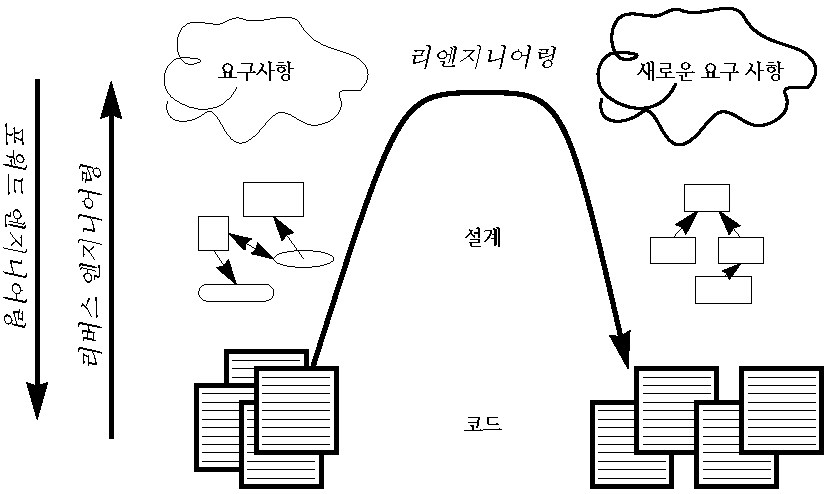
\includegraphics[width=\textwidth]{IntroLifecycle.pdf}
\caption{포워드 엔지니어링, 리버스 엔지니어링 그리고 리엔지니어링}
\figlabel{IntroLifecycle}
\end{center}
\end{figure}

\figref{IntroLifecycle}은 이 개념을 설명한다. \emph{포워드 엔지니어링(forward engineering)}은 높은 수준의 추상적인 모델과 아티팩트에서 구체적인 모델과 산출물로 이동하는 과정으로 이해할 수 있다. \emph{리버스 엔지니어링(reverse engineering)}은 코드에서 상위 수준의 모델과 산출물을 재구성한다. \emph{리엔지니어링(reengineering)}은 하나의 낮은 수준의 표현을 다른 표현으로 변환하는 과정이며, \emph{그 과정에서 상위 수준의 산출물을 다시 생성한다}. 

여기서 주목해야 할 핵심 사항은 리엔지니어링은 단순히 소스 코드를 변환하는 것이 아니라 시스템을 \emph{모든 수준}에서 변환하는 것이라는 점이다. 그렇기 때문에 리버스 엔지니어링과 리엔지니어링을 같은 맥락에서 이야기하는 것이 합리적이다. 일반적인 레거시 시스템에서는 소스 코드뿐만 아니라 모든 문서와 사양이 동기화되지 않은 것을 발견할 수 있다. 따라서 리버스 엔지니어링은 이해하지 못하는 것을 변형할 수 없기 때문에 리엔지니어링의 \emph{전제 조건(prerequisite)}이다.

%-----------------------------------------------------------------
\subsection*{리버스 엔지니어링}

무언가가 실제로 어떻게 작동하는지 이해하려고 할 때마다 \ind{리버스 엔지니어링(reverse engineering)}을 수행한다. 일반적으로 소프트웨어를 수정, 확장 또는 교체하려는 경우에만 리버스 엔지니어링이 필요하다. 소프트웨어를 리버스 엔지니어링해야 하는 이유는 때때로 \emph{사용 방법}을 이해하기 위해서일 수도 있다. 이는 리엔지니어링이 필요하다는 신호일 수도 있다. 따라서 리버스 엔지니어링 작업은 일반적으로 리엔지니어링에 대비해 소프트웨어를 \emph{재문서화(redocumenting)}하고 \emph{잠재적인 문제를 식별}하는 데 중점을 둔다.

리버스 엔지니어링을 하는 동안 다양한 정보 소스를 활용할 수 있다. 예를 들자면 다음과 같다.

\begin{bulletlist}

  \item 기존 문서 읽기

  \item 소스 코드 읽기

  \item 소프트웨어 실행해 보기

  \item 사용자 및 개발자 인터뷰하기

  \item 테스트 케이스 코딩 및 테스트 해보기

  \item 트레이스 생성 및 분석하기

  \item 다양한 도구로 소스 코드 및 트레이스의 하이 레벨 뷰(high-level views) 생성하기

  \item 버전 히스토리 분석하기
\end{bulletlist}

이러한 활동을 수행하면서 점진적으로 개선된 소프트웨어 모델을 구축하고, 다양한 질문과 답변을 찾고, 기술 문서를 정리하게 된다. 또한 수정해야 할 문제에 집중하게 될 것이다.

%-----------------------------------------------------------------
\subsection*{리엔지니어링}

시스템을 리엔지니어링하는 이유는 다양할 수 있지만, 실제 기술적인 문제는 일반적으로 매우 유사하다. 일반적으로 거시적인 아키텍처 문제와 세분화된 설계 문제가 혼합되어 있다. 대략적으로 문제를 분류해 보면 다음과 같다.

\begin{bulletlist}
  \item \emph{문서 부족(Insufficient documentation):}
  \index{문서!부족}
  문서가 존재하지 않거나 현실과 불일치한다.

  \item \emph{부적절한 레이어링(Improper layering):}
  \index{레이어링!부적절}
  누락되거나 부적절한 레이어링은 이식성(portability)과 적응성(adaptability)을 방해한다.

  \item \emph{모듈화 부족(Lack of modularity):}
  \index{모듈화!부족}
  모듈 간의 높은 결합도(couping)은 진화(evolution)를 방해한다.

  \item \emph{코드 중복(Duplicated code):}
  \index{코드 중복}
  ``복사, 붙여넣기 및 편집(copy, paste and edit)''은 빠르고 쉽지만 유지보수의 악몽(maintenance nightmares)으로 이어진다.

  \item \emph{기능 중복(Duplicated functionality):}
  \index{기능 중복}
  유사한 기능이 여러 팀에 의해 재구현되어 코드 비대화(code bloat)로 이어진다.
\end{bulletlist}

객체 지향 소프트웨어에서 발생하는 세분화된 가장 일반적인 문제는 다음과 같다.

\begin{bulletlist}
  \item \emph{상속의 오용(Misuse of inheritance):}
  \index{상속!오용}
  for composition, code reuse rather than polymorphism
  컴포지션(composition)의 경우 다형성(polymorphism)이 아닌 코드 재사용(code reuse)

  \item \emph{상속 누락(Missing inheritance):}
  \index{상속!누락}
  중복 코드(duplicated code)와 case 문에서 동작 선택하기 

  \item \emph{잘못 위치한 오퍼레이션(Misplaced operations):}
  \index{잘못 위치한 오펴레이션}
  잘못된 응집력(cohesion)\,---\,클래스 내부가 아닌 외부의 오퍼레이션의 위치

  \item \emph{캡슐화 위반(Violation of encapsulation):}
  \seeindex{캡슐화 위반}{캡술화, 위반}
  \index{캡슐화!위반}
  명시적 형 변환, C++ ``friends'' . 

  \item \emph{클래스 남용(Class abuse):}
  \index{클래스 남용}
  낮은 응집력(cohesion)\,---\,클래스를 네임스페이스처럼 사용
\end{bulletlist}

마지막으로, 변경하거나 교체하려는 시스템의 모든 부분에 대한 테스트 케이스를 철저하게 개발하여 리엔지니어링 활동을 위한 코드 기반을 준비한다.

리엔지니어링에는 마찬가지로 여러 가지 상호 관련된 활동이 따른다. 물론 가장 중요한 것 중 하나는 시스템의 어떤 부분을 수리하고 어떤 부분을 교체해야 하는지 평가하는 것이다.

\index{치코프스키, 엘리엇}
\index{크로스, 제임스}
실제로 수행되는 코드 변환은 여러 가지 범주로 나뉜다. 치코프스키와 크로스에 따르면 다음과 같다.

\index{리스터럭처링!정의}
\begin{quotation}
\noindent
``\emph{리스터럭처링(Restructuring)}는 시스템의 외부 동작을 유지하면서 동일한 상대적 추상화 수준에서 한 표현 형식에서 다른 표현 형식으로 변환하는 것이다.''
\end{quotation}

리스트럭처링은 일반적으로 소스 코드 변환(예: 비정형 ``스파게티'' 코드에서 구조화된 코드 또는 ``고투리스(goto-less)'' 코드로 자동 변환)을 의미하지만 디자인 수준에서의 변환도 포함할 수 있다. 

\index{리팩터링!정의}
\emph{리팩토링(Refactoring)}은 객체 지향 맥락 내에서 리스트럭처링하는 것이다. 마틴 파울러는 이렇게 정의한다.

\index{파울러, 마틴}
\begin{quotation}
\noindent
``\emph{리팩터링(Refactoring)}은 코드의 외부 동작을 변경하지 않으면서 내부 구조를 개선하는 방식으로 소프트웨어 시스템을 변경하는 프로세스이다.''

\hfill --- 마틴 파울러, \cite{Fowl99a}
\end{quotation}

소프트웨어 ``리엔지니어링(reengineering)''과 소프트웨어 ``유지보수(maintenance)''의 차이를 구분하기 어려울 수 있다. \ind{IEEE}는 \ind{소프트웨어 유지보수}를 정의하기 위해 여러 가지 시도를 해왔으며, 여기에는 다음도 포함된다.

\index{소프트웨어 유지보수!정의}
\begin{quotation}
\noindent
``결함을 수정하거나 성능 또는 기타 속성을 개선하거나 변경된 환경에 맞게 제품을 조정하기 위해 납품 후 소프트웨어 제품을 수정하는 것''. 
\end{quotation}

대부분의 사람들은 '유지보수'는 일상적인 작업인 반면 '리엔지니어링'은 그림 1에서 볼 수 있듯이 시스템을 재구성하는 과감하고 대대적인 노력이라고 생각할 것이다.

그러나 리엔지니어링은 단지 삶의 한 방식이라고 주장하는 사람들도 있다. 조금 개발하고, 조금 리엔지니어링하고, 조금 더 개발하는 식으로 \cite{Beck00a}. 실제로 건강하고 유지 관리 가능한 소프트웨어 시스템을 확보하기 위해서는 \emph{지속적인} 리엔지니어링 문화가 필요하다는 개념을 뒷받침하는 좋은 증거가 있다.

\index{리엔지니어링!지속적인}
그러나 지속적인 리엔지니어링(continuous reengineering)은 아직 일반적인 실천법이 아니기 때문에 이 책에서는 주요 리엔지니어링 노력의 맥락에서 패턴을 제시한다. 그럼에도 불구하고 독자들은 여기서 소개하는 대부분의 기법이 소규모 반복(iteration)에서 리엔지니어링에도 적용될 수 있다는 점을 염두에 두어야 한다.

%=================================================================
\section{리엔지니어링 패턴}

\index{리엔지니어링 패턴}
\index{알렉산더, 크리스토퍼}
글의 형식으로서의 패턴은 건축가 크리스토퍼 알렉산더가 1977년 그의 획기적인 저서인 \emph{패턴 랭귀지(A Pattern Language)}에서 소개했다. 이 책에서 알렉산더와 그의 동료들은 방에서 건물과 도시에 이르기까지 다양한 종류의 물리적 구조물을 설계하는 체계적인 방법을 제시했다. 각 문제는 여러 가지 주요한 요구사항(force)을 해결하는 일반적인 해결책인 반복되는 \emph{패턴(patter)}의 형태를 제시했지만, 특정 상황에 따라 각 문제에 고유한 방식으로 적용되어야 한다. 각 패턴에서 제시된 실제 해법은 그다지 흥미롭지 않았고, 오히려 패턴이 전달하는 \emph{주요한 요구 사항(force)}과 \emph{트레이드오프(tradeoff)}에 대한 논의가 포함되어 있다.

패턴은 디자인 문제에 대한 반복적인 해결책을 문서화하는 방법으로 소프트웨어 커뮤니티에서 처음 채택되었다. 알렉산더의 패턴과 마찬가지로, 각 디자인 패턴에는 해결해야 할 여러 가지 주요한 요구사항과 패턴을 적용할 때 고려해야 할 여러 가지 트레이드오프가 포함되었다. 패턴은 전문가들이 사용하는 실제 기법뿐만 아니라 그 뒤에 숨은 동기와 근거를 전달하는 간결한 방법인 것으로 밝혀졌다. 이후 패턴은 디자인 이외의 소프트웨어 개발의 여러 측면, 특히 소프트웨어를 설계하고 개발하는 \emph{프로세스(process)}에 적용되었다.

리엔지니어링 프로세스는 다른 프로세스와 마찬가지로 많은 표준 기법이 등장했으며, 각 기법은 다양한 주요한 요구사항을 해결하고 많은 트레이드오프를 포함할 수 있다. 모범 사례를 전달하는 방법으로서의 패턴은 이러한 기법을 제시하고 논의하는 데 특히 적합하다. 

\emph{리엔지니어링 패턴(reengineering patterns)}은 레거시 소프트웨어 수정에 관한 지식을 체계화하고 기록하여 문제를 진단하고 시스템의 추가 개발을 방해할 수 있는 약점을 파악하는 데 도움이 되며, 새로운 요구 사항에 더 적합한 솔루션을 찾는 데도 도움이 된다. \ind{리엔지니어링 패턴}은 모든 리엔지니어링 작업에서 참조할 수 있는 안정적인 전문 지식 단위로, 완전한 방법론을 제안하지 않고 프로세스를 설명하며 특정 도구를 ``판매''하려는 것보다는 적절한 도구를 제안한다. 

리버스 엔지니어링 및 리엔지니어링 패턴의 대부분은 소프트웨어 설계와 관련이 있다는 점에서 디자인 패턴과 표면적으로 유사하다. 그러나 디자인 패턴은 디자인 문제에 대한 특정 해결책을 선택하는 것과 관련이 있는 반면, 리엔지니어링 패턴은 \emph{기존 디자인을 발견(discovering an existing design)}하고, 어떤 \emph{문제(problem)}가 있는지 파악하고, 이러한 \emph{문제를 해결(reparing)}하는 것과 관련이 있다는 점에서 중요한 차이가 있다. 결과적으로 리엔지니어링 패턴은 순전히 주어진 디자인 구조보다는 \emph{발견과 변형의 프로세스(process of discovery and transformation)}와 더 관련이 있다. 이러한 이유로 이 책에 나오는 대부분의 패턴의 이름은 \patpgref{어뎁터}{Adapter} 또는 \patpgref{파사드}{Facade}와 같이 구조 지향적이기보다는 \patpgref{항상 실행 버전 보유하기}{AlwaysHaveARunningVersion}와 같이 프로세스 지향적이다. 

디자인 패턴이 반복되는 \emph{디자인(design)} 문제에 대한 해결책을 제시하는 반면, 리엔지니어링 패턴은 반복되는 \emph{리엔지니어링(reengineering)} 문제에 대한 해결책을 제시한다. 리엔지니어링 패턴으로 생성되는 산출물이 반드시 디자인일 필요는 없다. 리팩터링된 코드처럼 구체적일 수도 있고, 리버스 엔지니어링 패턴의 경우 시스템 작동 방식에 대한 인사이트처럼 추상적일 수도 있다.

좋은 리엔지니어링 패턴의 특징은 (a) 기존 시스템 상태와 비교하여 목표 산출물의 장점, 비용 및 결과를 명확하게 드러내는 것이지, 그 결과가 얼마나 우아한지가 \emph{아닌} 것이고, (b) 리엔지니어링 \emph{프로세스(process)}에 대한 설명, 즉 시스템의 한 상태에서 다른 상태로 이동하는 방법을 명확하게 설명하는 것이다.

리엔지니어링 패턴은 코드 리팩터링 그 이상을 포함한다. 리엔지니어링 패턴은 증상을 감지하는 것으로 시작하여 새로운 솔루션에 도달하기 위한 코드 리팩터링으로 끝나는 프로세스를 설명할 수 있다. 리팩터링은 이 프로세스의 마지막 단계에 불과하며, 새로운 솔루션을 구현하기 위해 코드를 자동 또는 반자동으로 수정하는 기술적 문제를 해결한다. 리엔지니어링 패턴에는 리팩터링의 일부가 아닌 다른 요소도 포함되는데, 리엔지니어가 직면하고 있는 제약 조건을 고려하여 증상의 맥락을 강조하고 리팩터링된 솔루션이 가져올 수 있는 변경의 영향에 대한 논의가 여기에 포함된다. 
%=================================================================
\section{리엔지니어링 패턴의 형식}

\begin{figure}
\begin{center}
\includegraphics[width=\textwidth]{IntroEg}
\caption{일반적인 리엔지니어링 패턴의 포맷}
\figlabel{IntroEg}
\end{center}
\end{figure}
(TODO: PNG 파일 처리 필요 혹은 현상태 유지)

\index{리엔지니어링 패턴!형식}
이 책에서 사용하는 형식(form)을 설명하는 간단한 패턴의 예가 \figref{IntroEg}에 나와 있다. 패턴마다 다른 종류의 문제를 다루기 때문에 실제 사용되는 형식은 패턴마다 약간 다를 수 있지만 일반적으로 같은 종류의 큰제목(heading)을 볼 수 있다.

패턴의 이름(name)은 잘 선택하면 패턴을 기억하기 쉽고 동료들과 토론하기 쉽게 한다. (''\patref{이해를 위한 리팩터링}{RefactorToUnderstand}을 하지 않으면 여기서 무슨 일이 일어나고 있는지 알 수 없을 것 같다.'') 의도(intent)는 패턴의 본질을 매우 간결하게 전달하고 현재 상황에 적용 가능한지 여부를 알려주어야 한다. 

많은 리엔지니어링 패턴은 코드 변환과 관련이 있으며, 이 경우 다이어그램을 사용하여 어떤 종류의 변환이 일어나는지 설명할 수 있다. 일반적으로 이러한 패턴에는 해결해야 할 문제를 감지하는 단계와 변환 전후의 상황을 보여주는 코드 조각이 추가로 포함된다.

%=================================================================
\section{리엔지니어링 패턴 지도}

\begin{figure}
\begin{center}
\includegraphics[width=\textwidth]{IntroMap}
\caption{리엔지니어링 패턴의 클러스터 지도}
\figlabel{IntroMap}
\end{center}
\end{figure}

이 책의 패턴은 앞서 제시한 리엔지니어링 라이프사이클(reengineering lifecycle)에 따라 정리되어 있다. 그림 3에서 이 책의 각 챕터가 라이프사이클에 따라 패턴의 클러스터로 표현된 것을 볼 수 있다. 이 다이어그램은 패턴이 순서대로 적용될 수 있음을 시사한다. 하지만 실제로는 리버스 엔지니어링과 리엔지니어링 작업을 반복할 가능성이 더 높다. 이 다이어그램은 '워터폴(Waterfall)' 라이프사이클이 단순한 것과 같은 의미에서 단순하다. 비록 순차적으로 수행되지 않고 반복적으로 수행된다는 것을 알고 있더라도 다양한 소프트웨어 엔지니어링 활동과 그 관계를 추적하는 데 유용한 방법이 될 수 있다.

\index{패턴!언어}
각 패턴 클러스터(cluster of patterns)는 공통의 문제 집합을 해결하기 위해 결합될 수 있는 관련 패턴의 집합인 간단한 ``패턴 언어(pattern language)''\,---\로 표시된다. 따라서 각 장은 일반적으로 해당 장의 패턴에 대한 개요와 맵으로 시작하여 패턴이 어떻게 연관될 수 있는지 제안한다.

\on{FIX -- need chapter links}

\charef{방향 설정}{SettingDirection}에는 리엔지니어링 노력의 초점을 어디에 맞출지 결정하고 진행 상황을 파악하는 데 도움이 되는 몇 가지 패턴이 포함되어 있다. \charef{첫 번째 접근}{FirstContact}은 레거시 시스템을 처음 접할 때 유용할 수 있는 패턴 집합으로 구성되어 있다. \charef{초기 이해}{InitialUnderstanding}는 주로 클래스 다이어그램의 형태로 레거시 시스템의 첫 번째 간단한 모델을 개발하는 데 도움이 된다. \charef{디테일한 모델 캡처}{DetailedModelCapture}는 시스템의 특정 구성 요소에 대한 보다 상세한 모델을 개발하는 데 도움이 된다.

\charef{테스트라는 생명보험}{TestsYourLifeInsurance}는 레거시 시스템을 이해하는 데 도움이 될 뿐만 아니라 리엔지니어링 작업에 대비하기 위해 테스트를 사용하는 데 중점을 둔다. \charef{마이그레이션 전략}{MigrationStrategies}은 리엔지니어링하는 동안 시스템을 계속 실행하고 새 시스템이 사용자에게 받아들여질 가능성을 높이는 데 도움이 된다. \charef{중복 코드 감지}{DetectingDuplicatedCode}는 다른 버전의 소프트웨어에서 코드를 복사하여 붙여넣거나 병합했을 수 있는 위치를 식별하는 데 도움이 될 수 있다. \charef{책임 재배포}{RedistributeResponsibilities}는 너무 많은 책임을 가진 클래스를 발견하고 리엔지니어링하는 데 도움이 된다. \charef{다형성 적용한 조건문 변환}{TransformConditionalsToPolymorphism}은 객체 지향 디자인이 시간이 지남에 따라 손상된 경우 책임을 재분배하는 데 도움이 된다.

%=============================================================
\ifx\wholebook\relax\else
   \bibliographystyle{alpha}
   \bibliography{scg}
   \end{document}
\fi
%=============================================================
